\input{GHERheader2014.tex}
\parindent 0cm

\author[Alexander Barth, Aida Alvera-Azc\'{a}rate, Mohamed~Ouberdous, Charles~Troupin, Sylvain~Watelet \& Jean-Marie~Beckers]{Alexander Barth, Aida Alvera-Azc\'{a}rate, Mohamed~Ouberdous,\\
 Charles~Troupin, Sylvain~Watelet \& Jean-Marie~Beckers}
  
\title[]{\diva workshop 2014}
\subtitle{New developments}
\date{}
\begin{document}

\maketitlepage % defined in GHERheader2013.tex


\newcommand{\ignore}[1]{}

%%%% debut macro %%%%
\newenvironment{changemargin}[2]{\begin{list}{}{%
\setlength{\topsep}{0pt}%
\setlength{\leftmargin}{0pt}%
\setlength{\rightmargin}{0pt}%
\setlength{\listparindent}{\parindent}%
\setlength{\itemindent}{\parindent}%
\setlength{\parsep}{0pt plus 1pt}%
\addtolength{\leftmargin}{#1}%
\addtolength{\rightmargin}{#2}%
}\item }{\end{list}}
%%%% fin macro %%%%


\begin{frame}[c]
\frametitle{\diva developments: summary}

\begin{itemize}

\item<1-> Modernisation of the code structure. \hfill  \textcolor{Green}{OK}
 
\item<2-> Support for observations in NetCDF format \hfill \textcolor{Orange}{In progress}

\item<3-> Multivariate approach   \hfill  \textcolor{Green}{OK}

\item<4-> Non-Gaussian distributed variables \hfill  \textcolor{Green}{OK}

\item<5-> 4-dimensional generalisation \hfill  \textcolor{Green}{OK: \texttt{divand}}

\item<6-> Spatially correlated observations errors \hfill \textcolor{Orange}{In progress}

\end{itemize}

\end{frame}

\begin{frame}[t]
\frametitle{Past releases: 4.5.1 -- March 2013}

\important{New features:} from user feedback during \\
\diva workshop 2012 (\textit{Roumaillac})

\onslide*<1>{
\begin{figure}
\centering
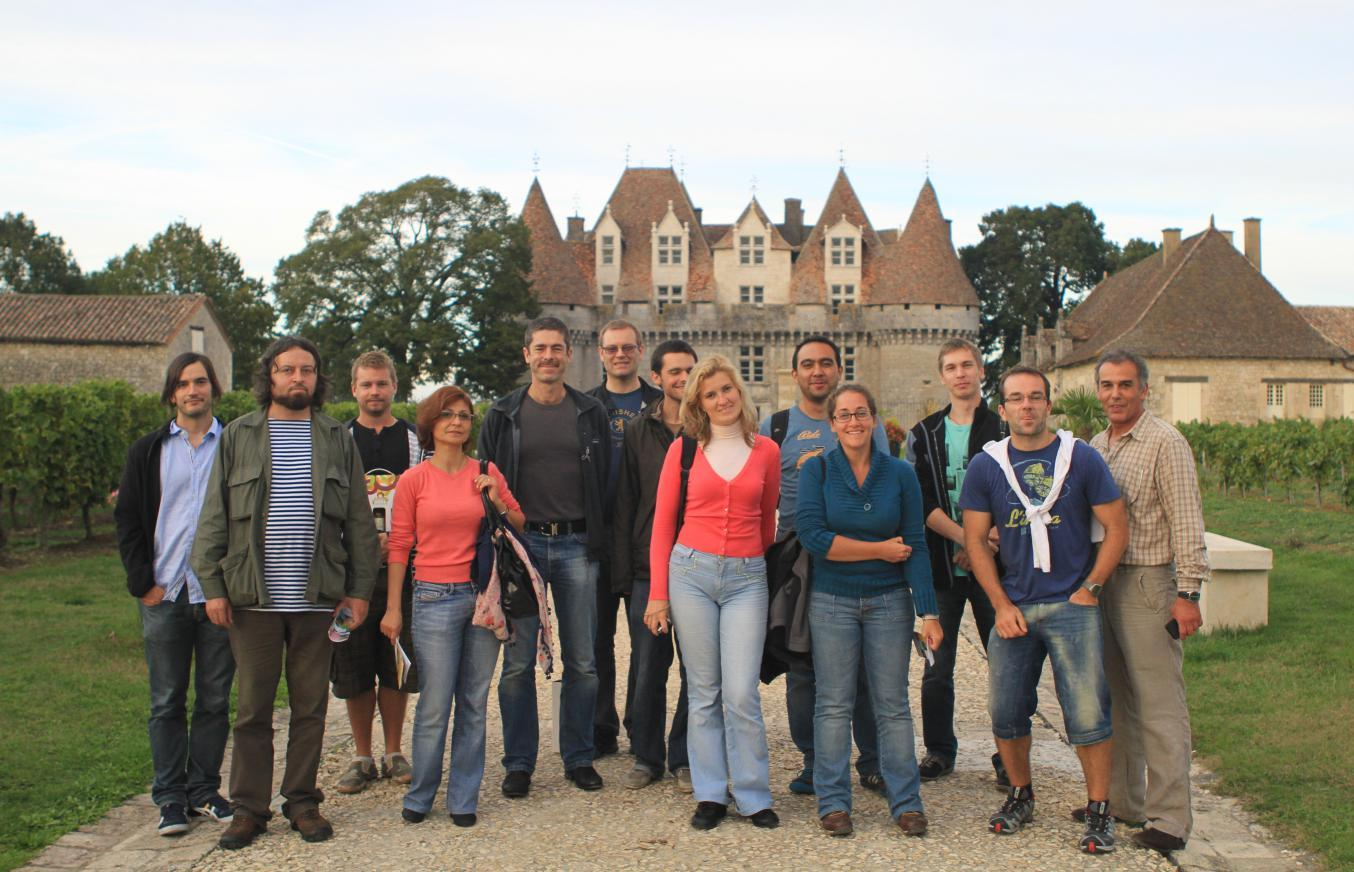
\includegraphics[width=.7\paperwidth]{Workshop2012}
\end{figure}
}

\begin{itemize}
\item<2-> Advection constraint with linear decay rate and local sources
\item<3-> \command{divadetrend}: change in the detrending order
\item<4-> Two new error calculations
\onslide*<4>{\begin{itemize}
\footnotesize
\item \command{divacpme}: quick \& better than original poor man's error
\item \command{divaexerr}: almost exact error calculation, much faster than the exact calculation
\end{itemize}
}
\item<5-> Simplified procedure for installation/compilation + tests
\item<6-> Housekeeping of the code \\
\onslide*<6>{
\footnotesize(simplifications, error messages, cleaning up of code, further optimisations, elimination of depreciated tools)
}
\item<7-> Updated user guide\\
\onslide*<7>{
\footnotesize(augmented with examples and new tool descriptions)
} 
\item<8-> Possibilities to call \diva from other software via system calls\\
\onslide*<7>{
\footnotesize(exemplified by a octave/matlab function \command{divagrid.m})
} 

\item<9-> \command{divadoxml} adapted to new specifications from IFREMER

\end{itemize}

\end{frame}

% -------------------------------------------------------------------------------------------------------------------------------------

\begin{frame}[t]
\frametitle{Past releases: 4.6.1 -- June 2013}


\begin{itemize}
\item<2-> Two additional solvers
\begin{itemize}
\item parallel version
\item iterative version
\end{itemize} 

\item<3-> Optimisations for large data sets
\item<4-> Optimisations of file exchanges for use with ODV
\item<5-> Highly optimised new version of the grid generator
\end{itemize} 
\end{frame}

% -------------------------------------------------------------------------------------------------------------------------------------

\begin{frame}[c]
\frametitle{Better, faster, stronger \ldots}


\vspace{-0.25cm}

\begin{columns}[totalwidth=1.1\textwidth]
\column{.2\textwidth}
\onslide*<1>{\important{Mesh:}\\
very fine meshes in a few seconds
}
\onslide*<2>{\important{Analysis:}\\
2 million data $\approx$ 1 minute}
\column{.9\textwidth}
\begin{figure}
\centering
\includegraphics<1>[height=.5\paperwidth]{Time_mesh}
\includegraphics<2>[height=.5\paperwidth]{Diva_time_2013_05_30_09_06_55_gfortran_4pt6}
\end{figure}
\end{columns}

\onslide*<3>{
\important{Solvers:} 
\begin{itemize}
\item Direct
\item Parallel
\item Iterative
\end{itemize}
}

\onslide*<4>{
\begin{center}
\important{Mesh:} $\approx$ 100 $\times$ faster\\
\important{Analysis:} $\approx$ 5-10 $\times$ faster

\vspace{1cm}

$\rightarrow$ also quicker in ODV 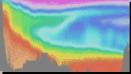
\includegraphics[height=.5cm]{odvico}
\end{center}
}

\end{frame}



% -------------------------------------------------------------------------------------------------------------------------------------
\begin{frame}[t]
\frametitle{Scientific developments -- innovations}

\vspace{.15cm}

\footnotesize

\begin{columns}[totalwidth=1.1\textwidth,t]
\column{.65\textwidth}


\onslide*<1>{\important{4-dimensional generalisation: \command{divand}} 
\vspace{1cm}
\begin{itemize}
\item Derivation of the kernel for $n$ dimensions
\item Additional constraint 
\item Algorithms (primal and dual formulations)
\end{itemize}
\vspace{1cm}

Released code version available at:\\
\url{http://modb.oce.ulg.ac.be/mediawiki/index.php/Divand}
}

\onslide*<2>{\important{Spatially correlated observations}

\vspace{1cm}

\begin{description}
\item[Ideally:] observation errors not correlated
\item[Reality:] clusters of observations (cruises, \ldots)
\item[Consequence:] observations error covariance matrix is not diagonal
\end{description}

}


\onslide*<3>{\important{New error computation}

\vspace{1cm}

\begin{description}
\item[Poor man's error:] quick, but error underestimation 
\item[Real covariance:] correct error estimation but very slow
\item[Now:] two quicker/more accurate methods
\end{description}

}
\onslide*<4>{\important{Adaptation to altimetry data}

\vspace{1cm}

\begin{itemize}
\item Particular temporal/spatial coverage
\item Input files: NetCDF
\item Modified data weights according to time of measurement
\end{itemize}

}

\onslide*<5>{\important{Python plotting tools}

\vspace{1cm}

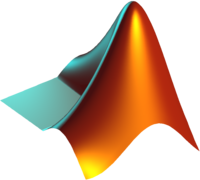
\includegraphics[height=.6cm]{Matlab_Logo}~\raisebox{0.2cm}{$\boldsymbol{\rightarrow}$}~
\includegraphics[height=.6cm]{pythonlogo}


\begin{itemize}
\item Free alternative to matlab/octave
\item Easily deals with NetCDF
\item Publication quality figures with Matplotlib
\end{itemize}
\vspace{1cm}
\url{http://modb.oce.ulg.ac.be/mediawiki/index.php/Diva_python}

}

\column{.45\textwidth}

\onslide*<1>{
\begin{figure}
{\footnotesize RMS 3D analysis}\\
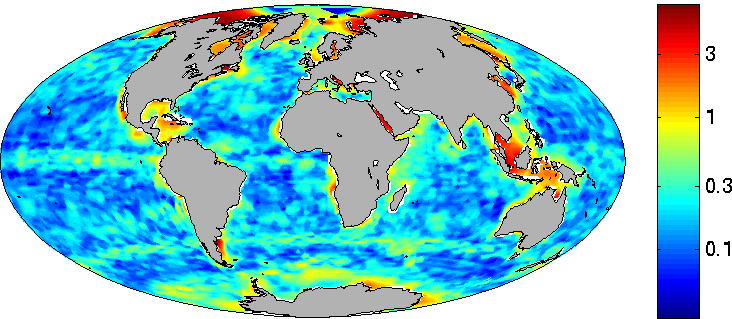
\includegraphics[width=.7\columnwidth]{orca_test_divand3_rms_3d}
\end{figure}
}

\onslide*<2>{

}

\onslide*<3>{
\begin{figure}
\centering
{\footnotesize Clever poor man's estimate}\\
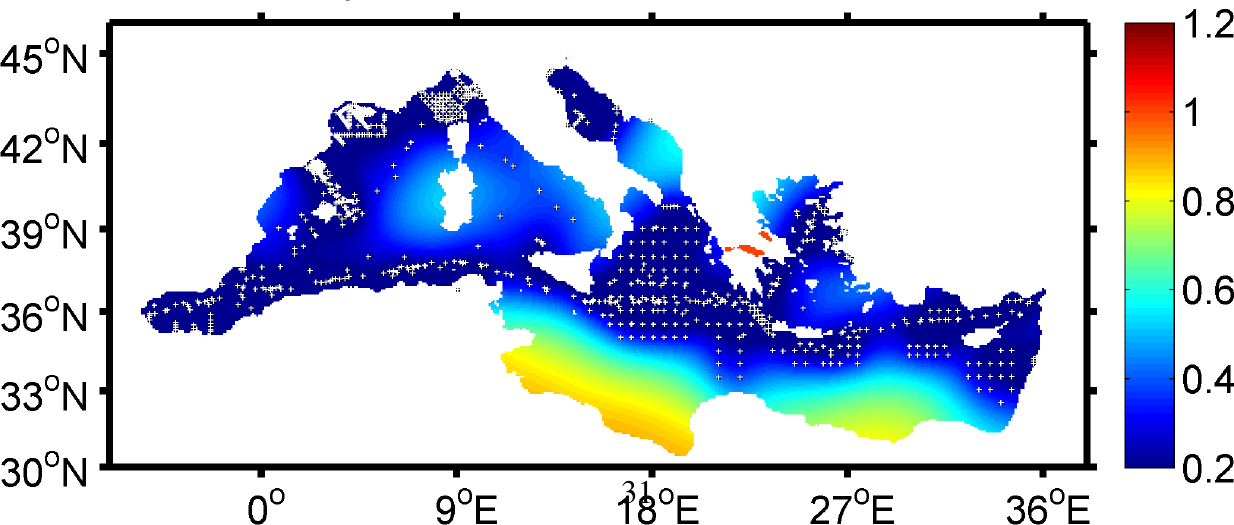
\includegraphics[width=.7\columnwidth]{error_med_cpm}\\
{\footnotesize Almost exact error}\\
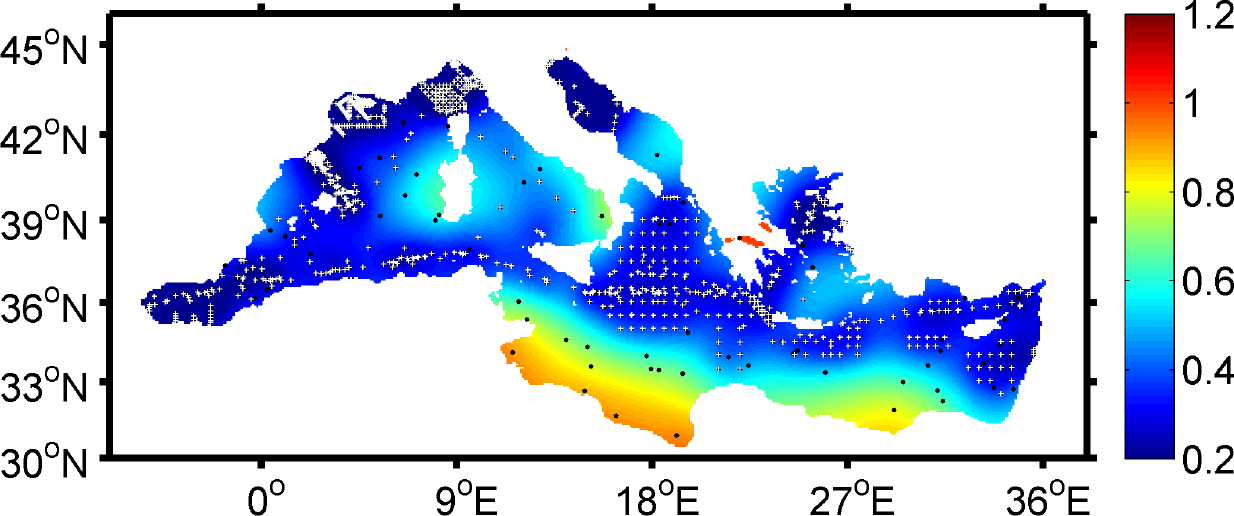
\includegraphics[width=.7\columnwidth]{error_med_exerr}
\end{figure}

}

\onslide*<4>{

\begin{figure}
\flushleft
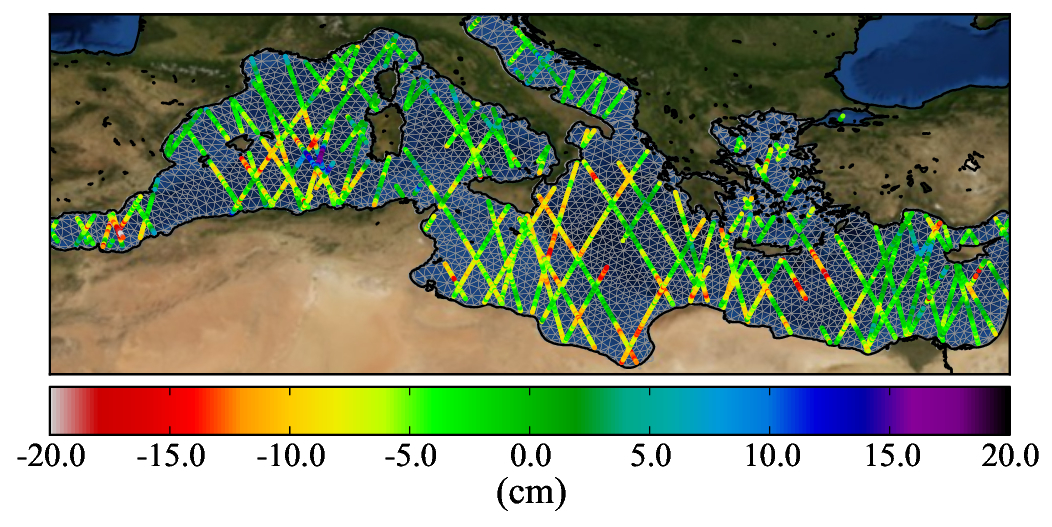
\includegraphics[width=.9\columnwidth]{dt_upd_med_en_j1n_j2_sla_vxxc_20090513_20090520_20100503_diva4.jpg}\\
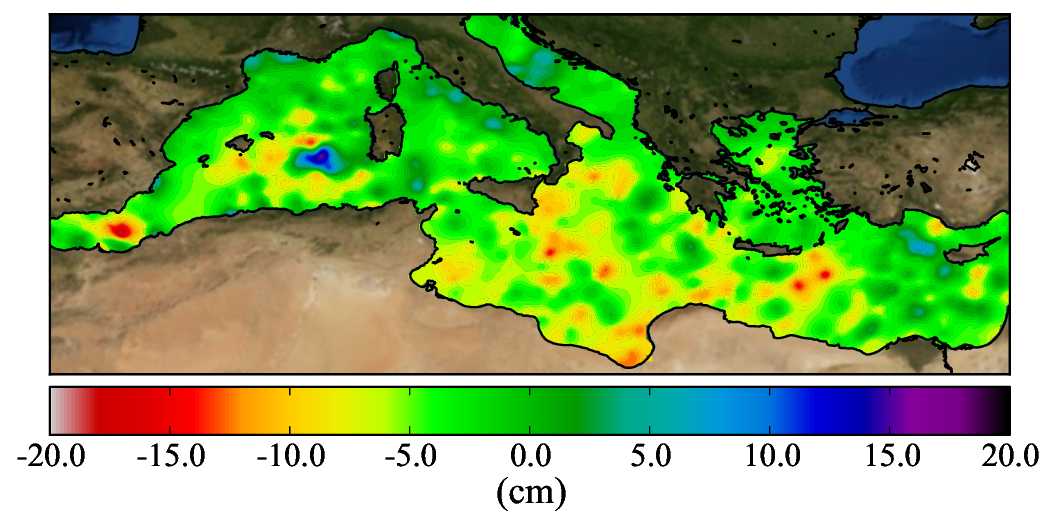
\includegraphics[width=.9\columnwidth]{dt_upd_med_en_j1n_j2_sla_vxxc_20090513_20090520_20100503_diva6.jpg}
\end{figure}

}

\onslide*<5>{
\begin{figure}
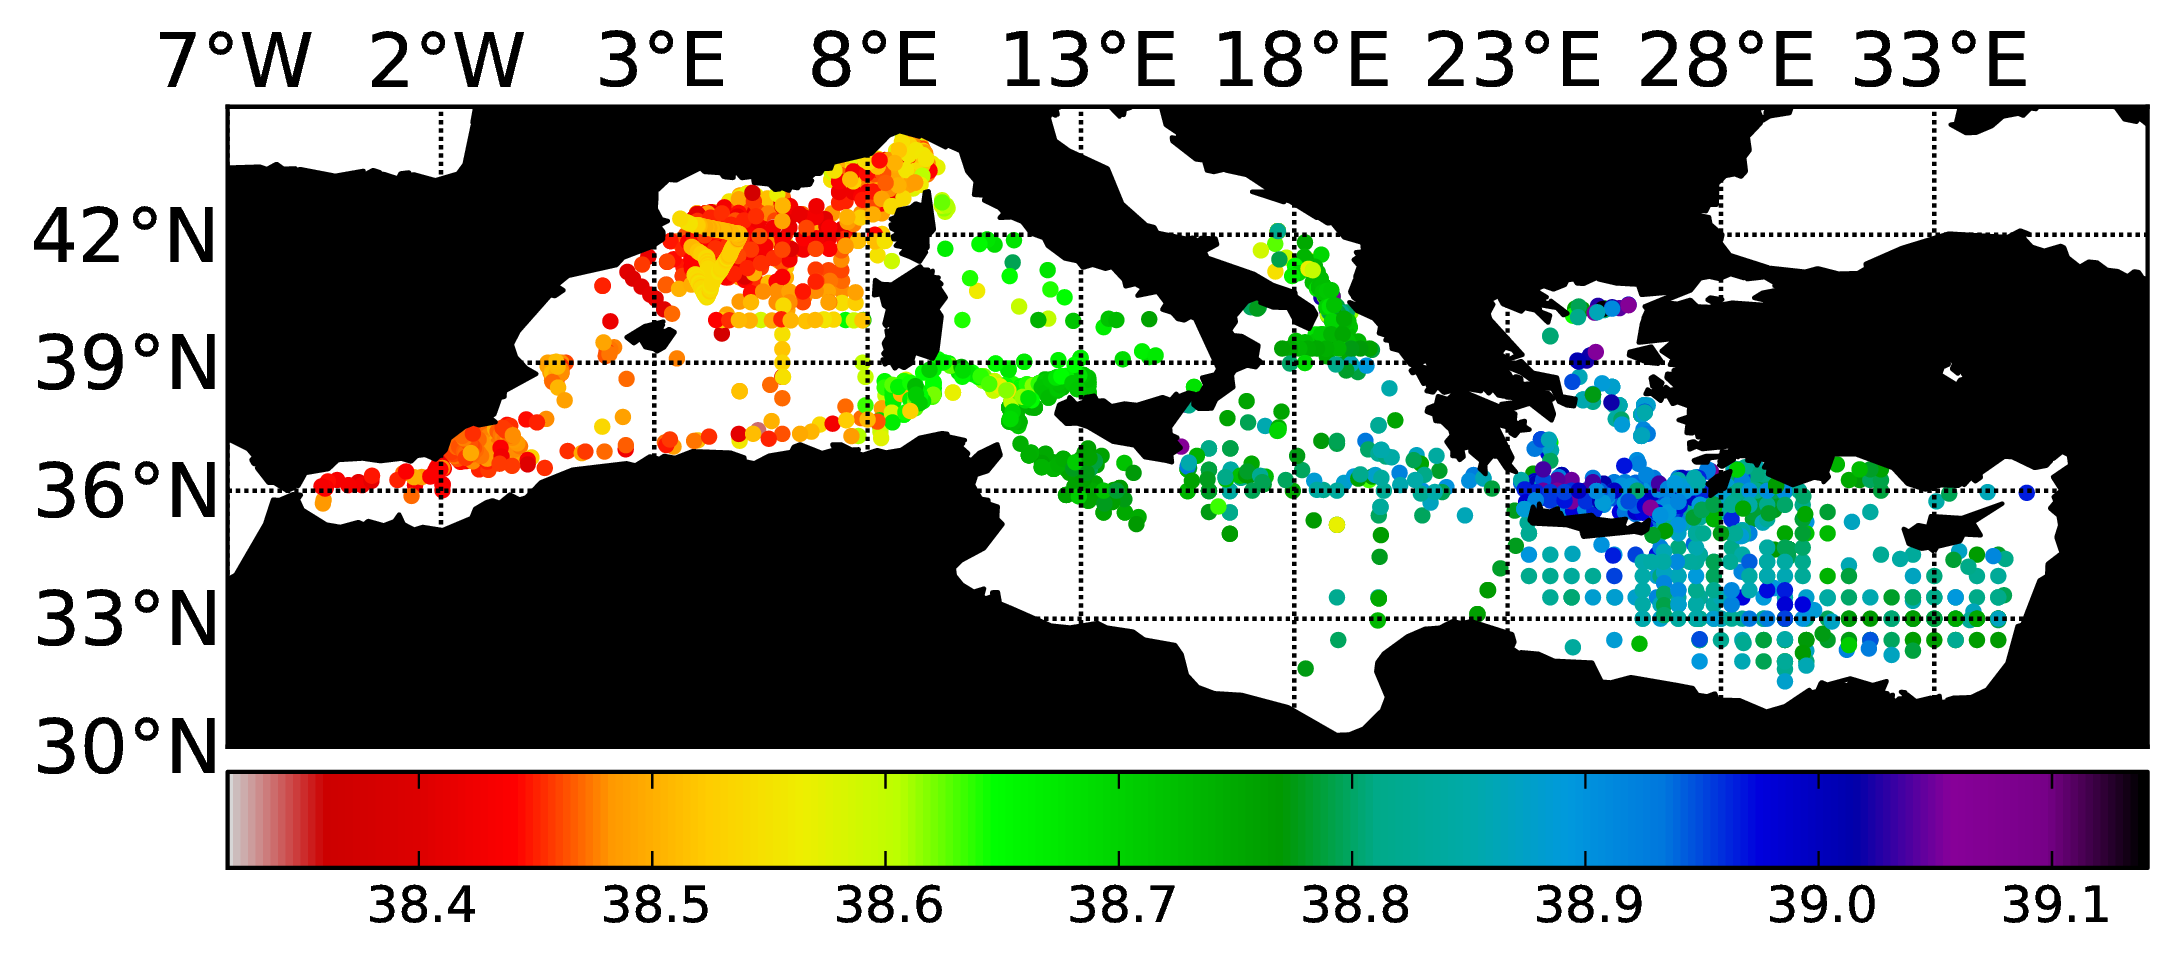
\includegraphics[width=.9\columnwidth]{Data_ex_py}\\
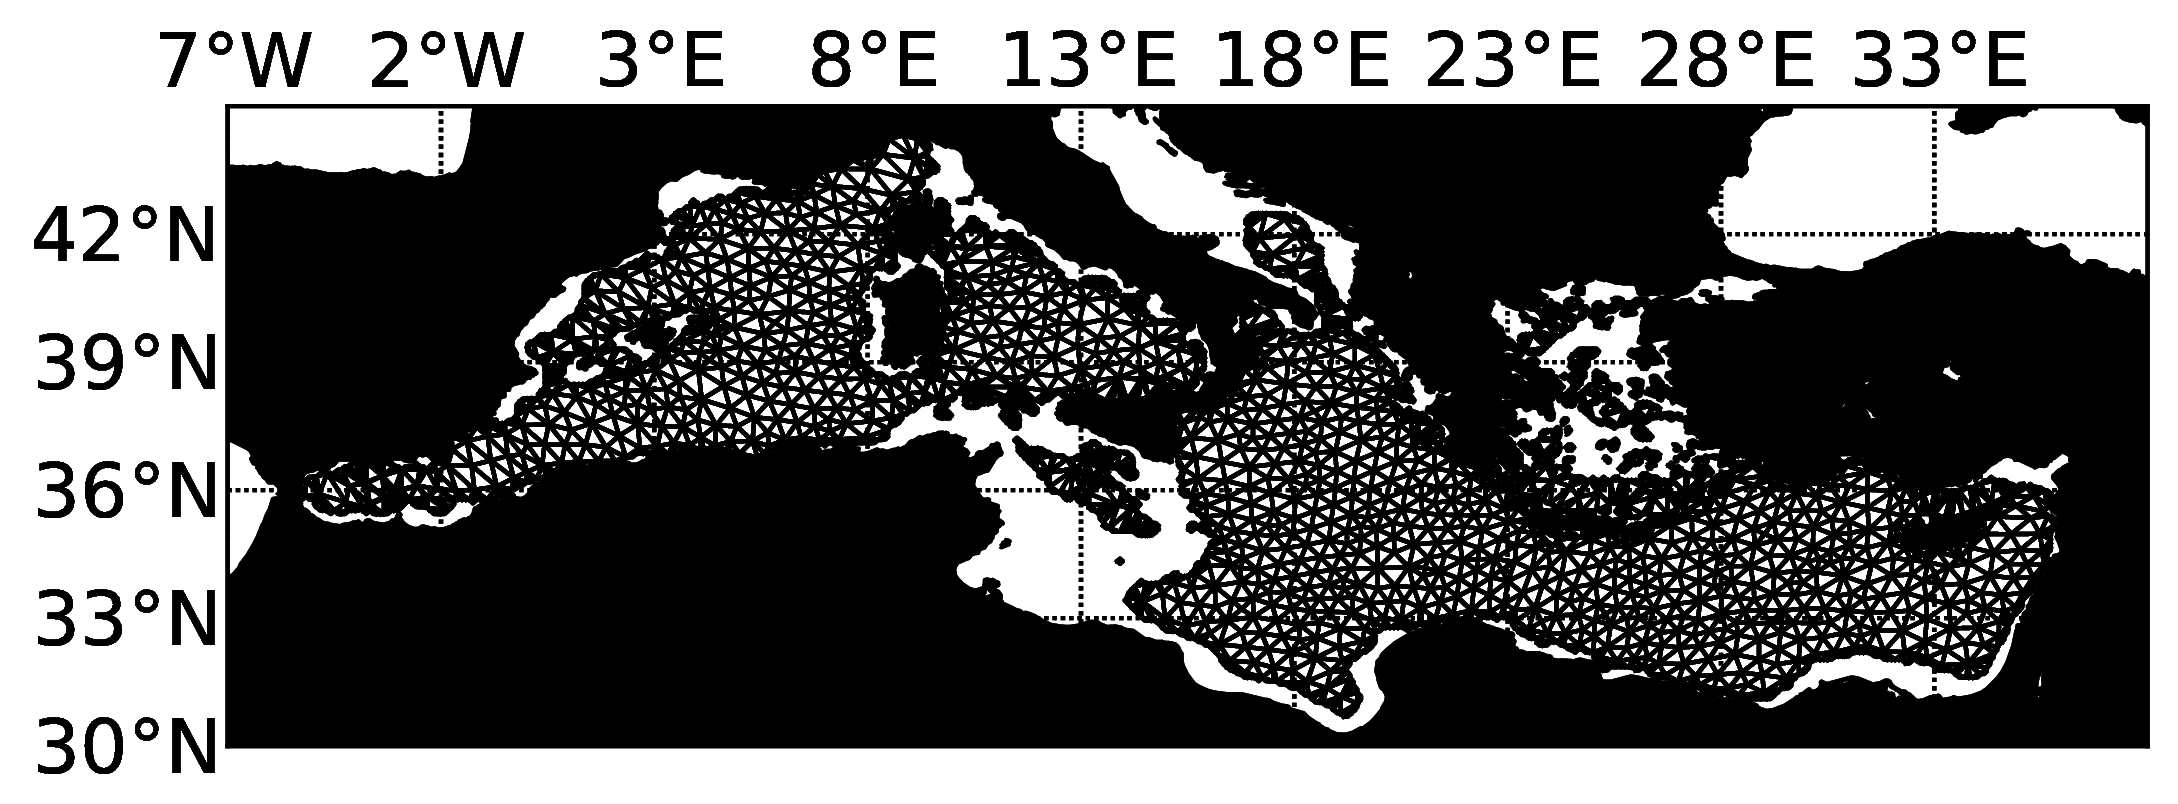
\includegraphics[width=.9\columnwidth]{Mesh_ex_py}\\
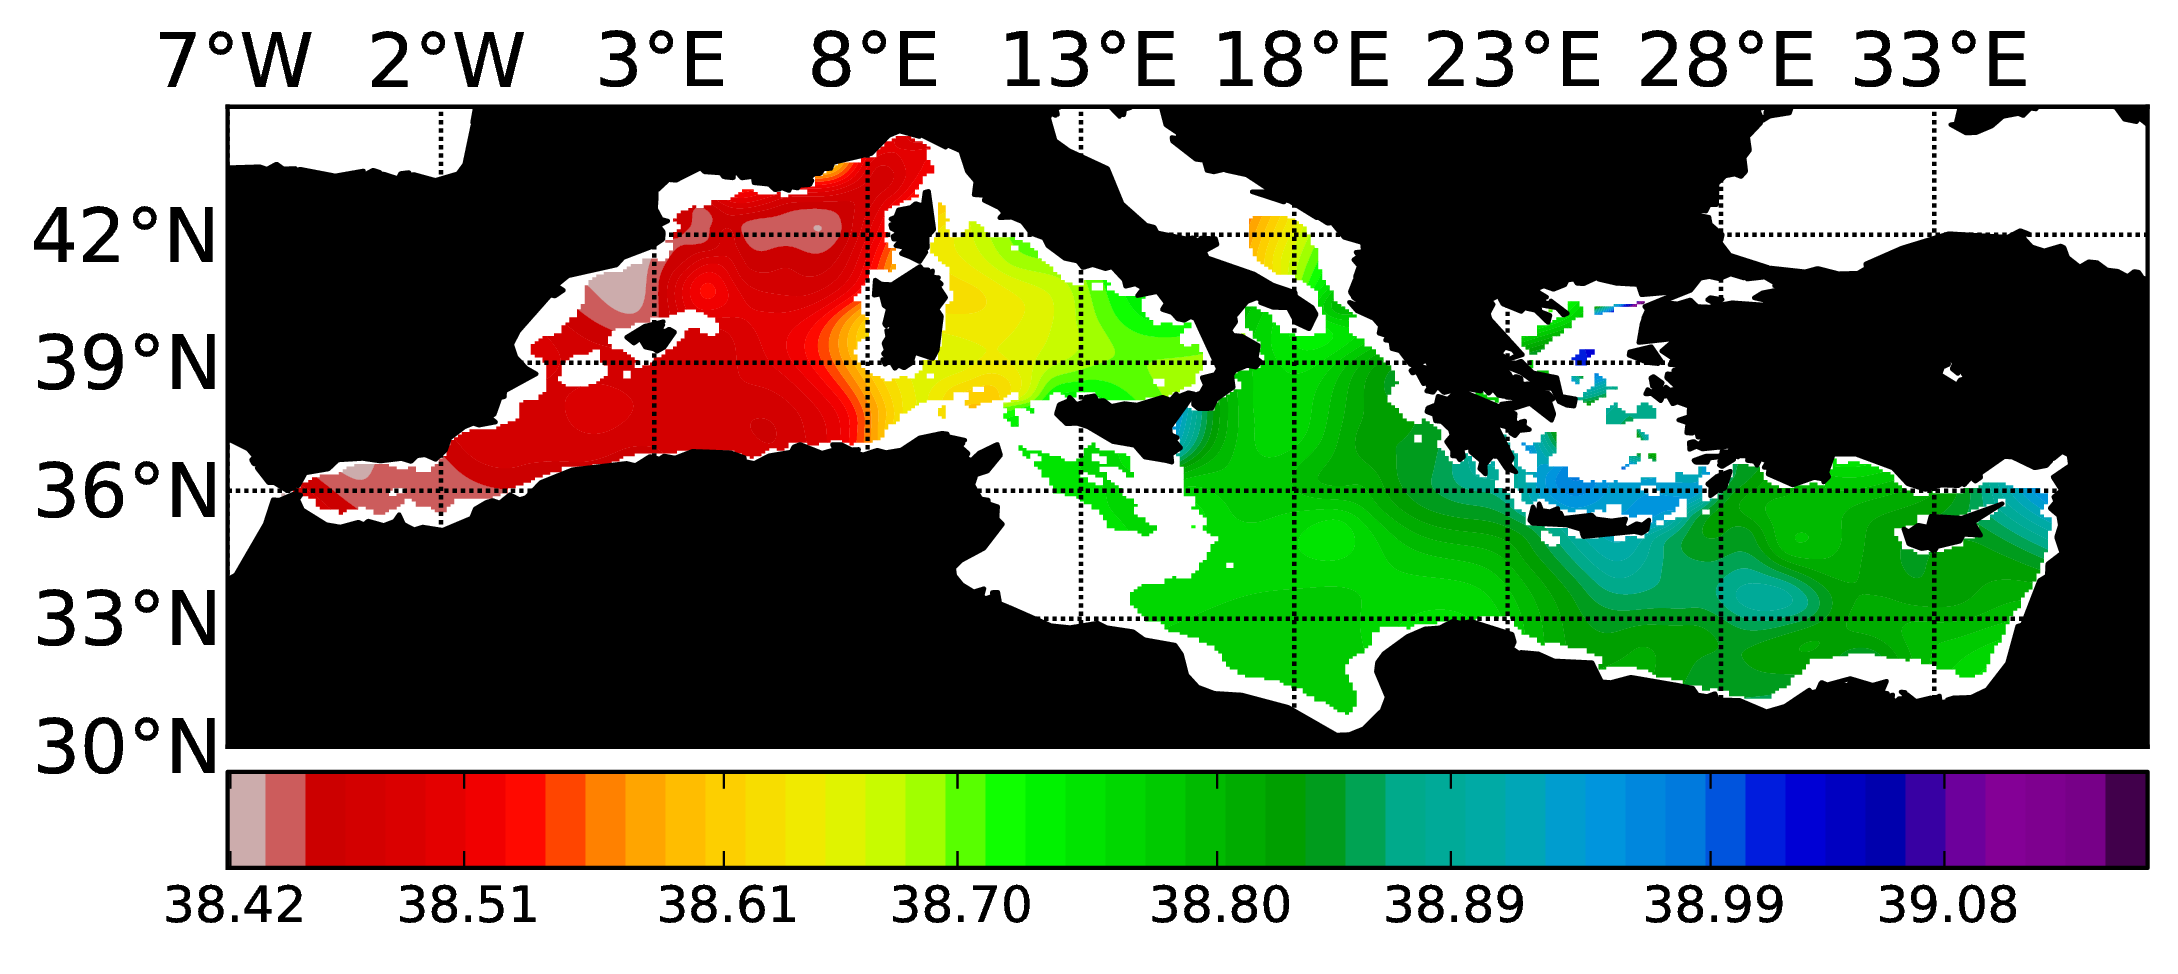
\includegraphics[width=.9\columnwidth]{Results_ex_py}
\end{figure}

}


\end{columns}

\end{frame}

% -------------------------------------------------------------------------------------------------------------------------------------
\begin{frame}
\frametitle{Publications}

\footnotesize

\begin{columns}[totalwidth=1.1\textwidth]
\column{.65\textwidth}


\onslide*<1>{\important{Detrending:}
 
\vspace{1cm}

\method{Recognizing temporal trends in spatial interpolation : an
application to the Black Sea Cold Intermediate Layer and
mixed layer depth}\\
A.~Capet, C.~Troupin, J.~Carstensen, M.~Gr\'{e}goire \& J.-M.~Beckers\\
\textit{Ocean Dynamics}\\
Under revision
}

\onslide*<2>{\important{Diva-nd:}

\vspace{1cm}

\method{divand-1.0: n-dimensional variational data analysis for ocean observations}\\
A.~Barth, J.-M.~Beckers, C.~Troupin, A.~Alvera-Azc\'{a}rate \& L.~Vandenbulcke\\
\textit{Geoscientific Model Development}\\
Under revision
}


\onslide*<3>{\important{Error field:}


\vspace{1cm}

\method{Approximate and efficient methods to assess error fields in spatial gridding with \diva
(Data Interpolating Variational Analysis)}\\
J.-M.~Beckers, A.~Barth, C.~Troupin \& A.~Alvera-Azc\'{a}rate\\
\textit{Journal of Atmospheric and Oceanic Technology}\\
Under revision
}

\column{.45\textwidth}

\onslide*<1>{
\begin{figure}
\centering
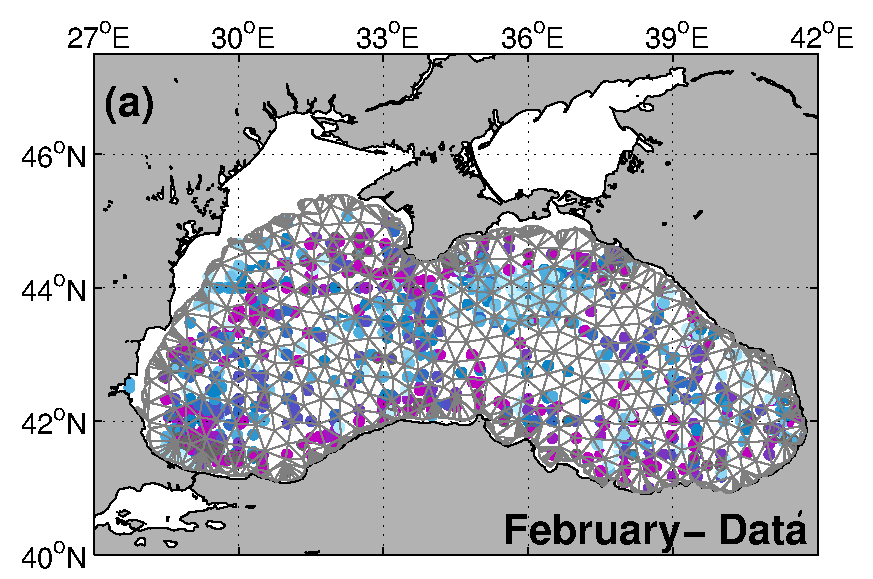
\includegraphics[width=.65\columnwidth]{2012gl055036-p02a}\\
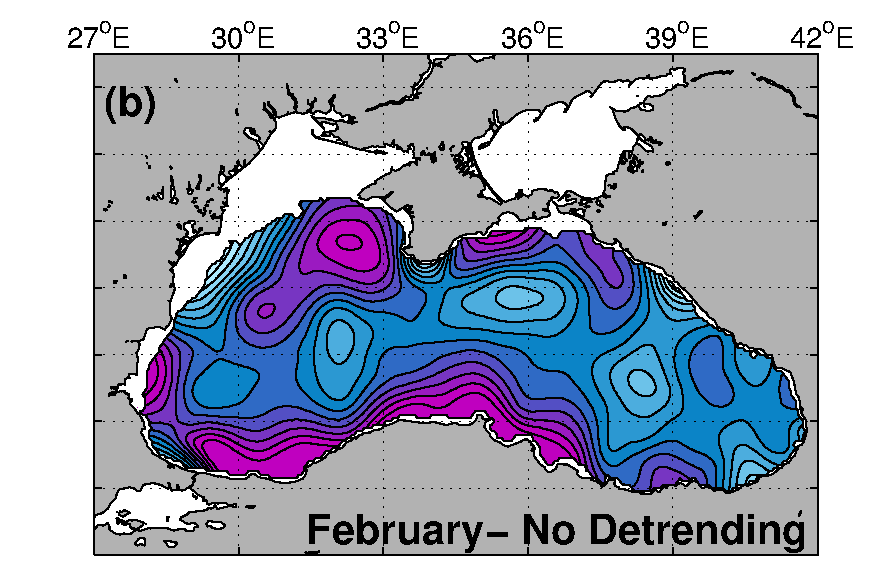
\includegraphics[width=.65\columnwidth]{2012gl055036-p02b}\\
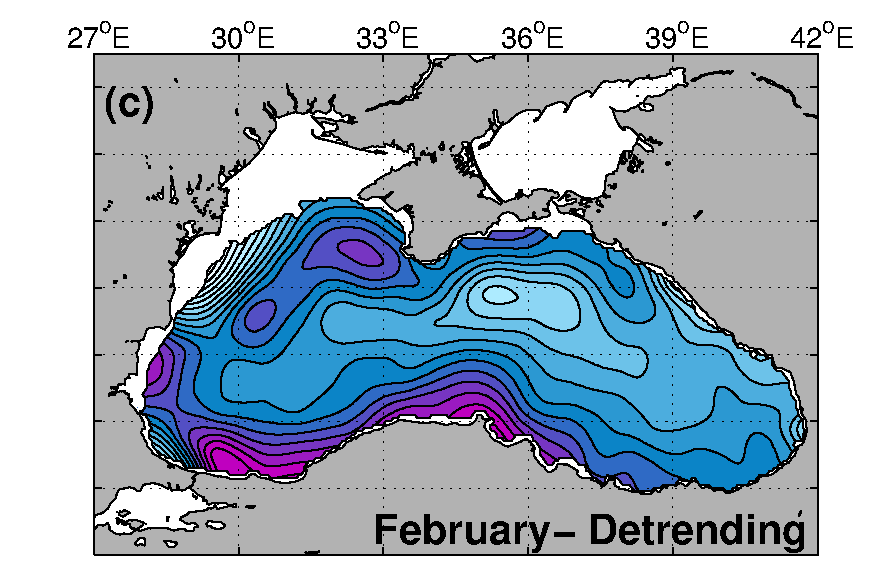
\includegraphics[width=.65\columnwidth]{2012gl055036-p02c}
\end{figure}
}

\onslide*<2>{
\begin{figure}
\centering
{\footnotesize RMS 2D analysis}\\
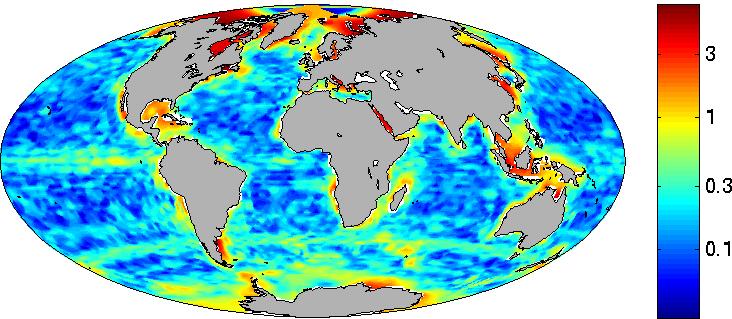
\includegraphics[width=.7\columnwidth]{orca_test_divand3_rms_2d}\\
{\footnotesize RMS 3D analysis}\\
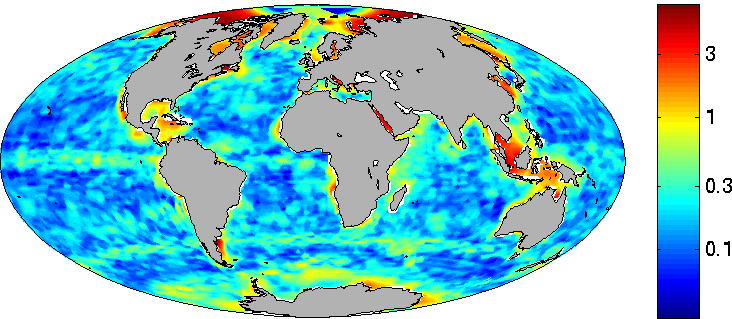
\includegraphics[width=.7\columnwidth]{orca_test_divand3_rms_3d}\\
{\footnotesize RMS(2D) -- RMS(3D)}\\
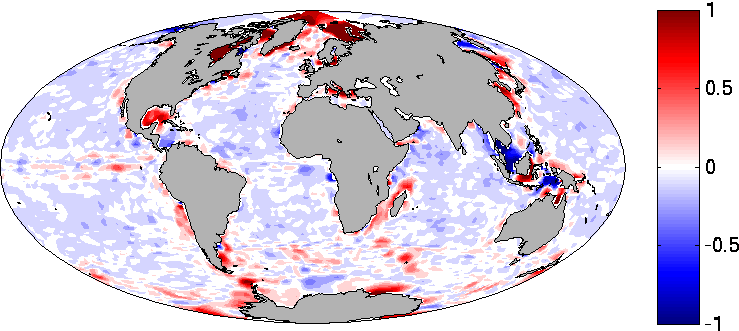
\includegraphics[width=.7\columnwidth]{orca_test_divand3_rms_3d2d}
\end{figure}
}

\onslide*<3>{
\begin{figure}
\centering

{\footnotesize Real covariance}\\
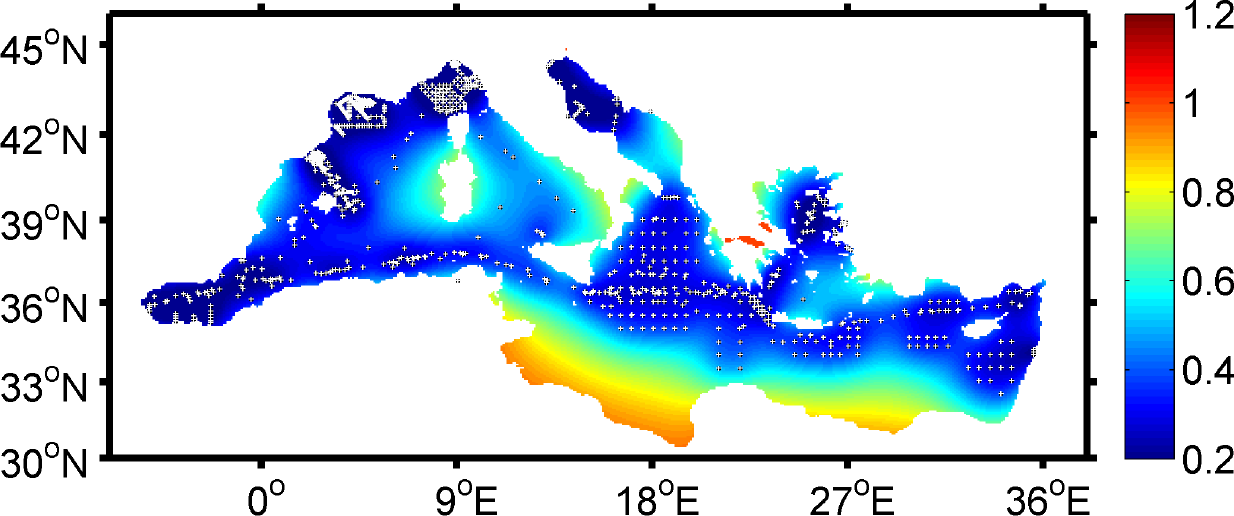
\includegraphics[width=.7\columnwidth]{error_med_real}\\
{\footnotesize Clever poor man's estimate}\\
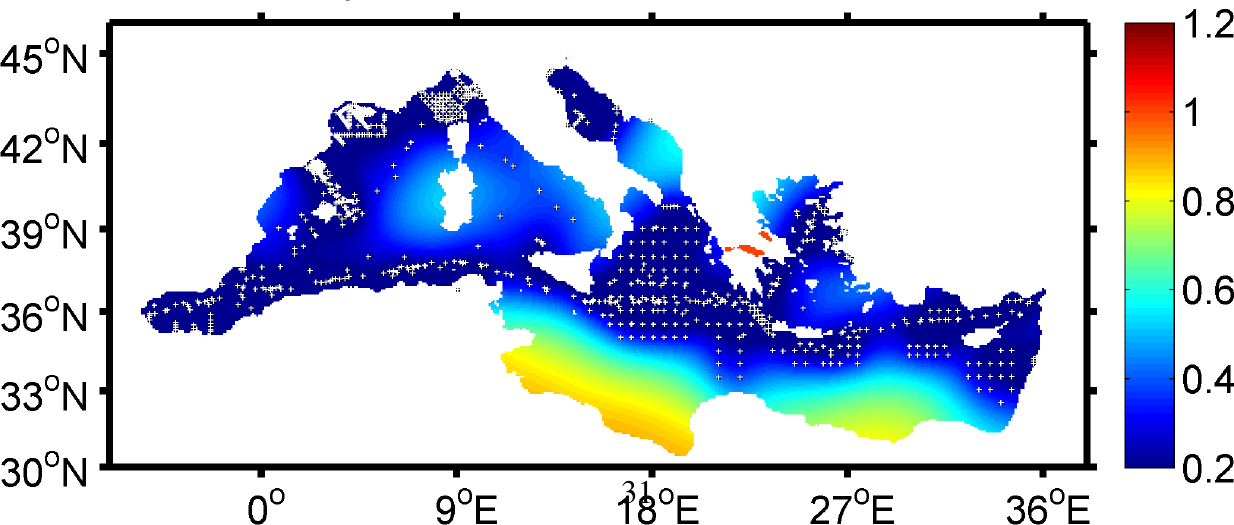
\includegraphics[width=.7\columnwidth]{error_med_cpm}\\
{\footnotesize Almost exact error}\\
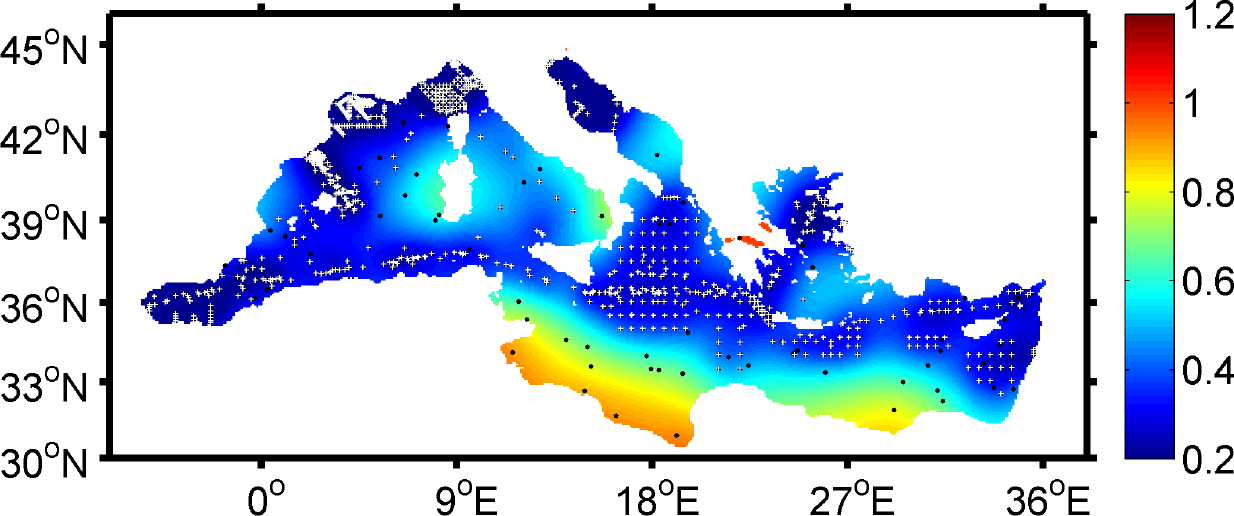
\includegraphics[width=.7\columnwidth]{error_med_exerr}
\end{figure}
}



\end{columns}

\end{frame}

%--------------------------------------------------------------------------------------------------------
\begin{frame}[fragile]
\frametitle{DivaonedepthODV4}
\framesubtitle{Introduction}

Purpose : \textbf{Handling of files with \textcolor{red}{no vertical axis}}

\pause

\begin{itemize}
 \item For instance, a BODC file :
\end{itemize}

\begin{changemargin}{-0.9cm}{0cm}
\begin{tiny}
\begin{verbatim}
//Data documentation at http://www.bodc.ac.uk/data/documents/series/7011/
//SDN_parameter_mapping
//<subject>SDN:LOCAL:Chronological Julian Date</subject><object>
SDN:P011::CJDY1101</object><units>SDN:P061::UTAA</units>
//<subject>SDN:LOCAL:CurrDir</subject><object>SDN:P011::
LCDAEL01</object><units>SDN:P061::UABB</units>
//<subject>SDN:LOCAL:CurrSpd</subject><object>SDN:P011::
LCSAEL01</object><units>SDN:P061::UVBB</units>
//

Cruise Station Type yyyy-mm-ddThh:mm:ss.sss Longitude [degrees_east] Latitude [degrees_north] 
LOCAL_CDI_ID EDMO_code Bot.Depth [m] Chronological Julian Date [days] QV:SEADATANET CurrDir [deg T] 
QV:SEADATANET   CurrSpd [cm/s]  QV:SEADATANET
PBISOP/SB1 B1/328/MB * 1971-08-30T10:31:00.000 -5.6166 54.9833 7011 43 148 2441194.438194 1 280.60 
1 4.90 1
        2441194.445139 1 266.90 1  5.50 1
        2441194.452083 1 193.00 1  6.70 1
        2441194.459027 1 185.40 1  9.50 1
        2441194.465972 1 176.60 1 13.50 1
        2441194.472916 1 174.00 1 15.30 1
        2441194.479861 1 170.50 1 18.10 1
               .       .    .   .   .   .
               .       .    .   .   .   .
               .       .    .   .   .   .
               .       .    .   .   .   .

\end{verbatim} 
\end{tiny}
\end{changemargin}

\end{frame}
%--------------------------------------------------------------------------------------------------------
\begin{frame}
\frametitle{DivaonedepthODV4}
\framesubtitle{Step 1 - Recognition}
The script performs several preliminary tests :
\begin{enumerate}
 \item pressure axis ? $\Rightarrow$ exit
 \item depth axis ? $\Rightarrow$ exit
 \item no metadata file ? $\Rightarrow$ exit + warning
 \item \textbf{else ?} $\Rightarrow$ file with \textbf{no vertical axis}
\end{enumerate}

\begin{center}
 -----------------------------
\end{center}

\begin{itemize}
 \item CurrDir, CurrSpd and a vertical axis ? $\Rightarrow$ special case (see later)
\end{itemize}


\end{frame}
%--------------------------------------------------------------------------------------------------------
\begin{frame}
\frametitle{DivaonedepthODV4}
\framesubtitle{Step 2 - Variables averaging}
\textbf{Scalar} variables
\begin{itemize}
 \item simple arithmetic average
\end{itemize}
~\\
\textbf{Vectorial} variable
\begin{itemize}
 \item only for current speed (currdir \& currspd) ($\rightarrow$ future upgrade)
 \item polar coordinate system $\Rightarrow$ Cartesian coordinate system (u\_star \& v\_star)
 \item simple arithmetic average
\end{itemize}


\end{frame}
%--------------------------------------------------------------------------------------------------------
\begin{frame}
\frametitle{DivaonedepthODV4}
\framesubtitle{Step 3 - Writing a new data file}

\emph{A new file\ldots}
\begin{itemize}
 \item The new file has the extension ``\textbf{\_bis}.txt'' instead of ``.txt''
 \item There are only two data line left, containing the mean values of the variables
 \item Currspd and Currdir become u\_star and v\_star
 \item A column ``Depth [m]'' is added
\end{itemize}

\pause
\vspace{0.2cm}

\emph{\ldots with a new depth axis}
\begin{enumerate}
\item the average of ``minimum instrument depth'' and ``maximum instrument depth'' is computed
\item the file ``contour.depth'' is read and the two nearest depths are written in the new file
\end{enumerate}


\end{frame}
%--------------------------------------------------------------------------------------------------------
\begin{frame}[fragile]
\frametitle{DivaonedepthODV4}
\framesubtitle{Step 3 - Writing a new data file}
A new file :
~\\
\begin{changemargin}{-0.9cm}{0cm}
\begin{tiny}
\begin{verbatim}
//Data documentation at http://www.bodc.ac.uk/data/documents/series/7011/
//SDN_parameter_mapping
//<subject>SDN:LOCAL:Chronological Julian Date</subject><object>
SDN:P011::CJDY1101</object><units>SDN:P061::UTAA</units>
//<subject>SDN:LOCAL:CurrDir</subject><object>SDN:P011::
LCDAEL01</object><units>SDN:P061::UABB</units>
//<subject>SDN:LOCAL:CurrSpd</subject><object>SDN:P011::
LCSAEL01</object><units>SDN:P061::UVBB</units>
//

Cruise Station Type yyyy-mm-ddThh:mm:ss.sss Longitude [degrees_east] Latitude [degrees_north] 
LOCAL_CDI_ID EDMO_code Bot.Depth [m] Chronological Julian Date [days] QV:SEADATANET u_star [cm/s]
QV:SEADATANET v_star [cm/s] QV:SEADATANET   Depth [m]
PBISOP/SB1 B1/328/MB * 1971-08-30T10:31:00.000 -5.6166 54.9833 7011 43 148 2441194.438194 1 
-10.02333087929292929292 1 3.46943974242424242424  1 150
        2441194.445139 1 -10.02333087929292929292 1 3.46943974242424242424 1 100
\end{verbatim} 
\end{tiny}
\end{changemargin}

\vspace{-1.2cm}
\hspace{4.5cm}
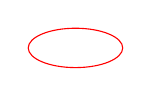
\begin{tikzpicture}
\draw[red] (0,0) ellipse (0.6cm and 0.25cm);
\end{tikzpicture}
\vspace{1.2cm}

\vspace{-1.25cm}
\hspace{5.6cm}
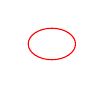
\begin{tikzpicture}
\draw[red] (0,0) ellipse (0.3cm and 0.2cm);
\end{tikzpicture}
\vspace{1.25cm}

\vspace{-1.45cm}
\hspace{8.65cm}
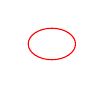
\begin{tikzpicture}
\draw[red] (0,0) ellipse (0.3cm and 0.2cm);
\end{tikzpicture}
\vspace{0.8cm}

The following files are also modified :
\begin{description}
 \item[varlist]u\_star and v\_star are added to the list
 \item[datasource]the old files are replaced by the new ones (``\_bis'')
\end{description}
\end{frame}
%--------------------------------------------------------------------------------------------------------
\begin{frame}
\frametitle{DivaonedepthODV4}
\framesubtitle{Other features}
\textbf{Tests and warnings}
\begin{itemize}
 \item no depth in the metadata file $\Rightarrow$ exit + warning
 \item more than one scalar variable $\Rightarrow$ exit + warning ($\rightarrow$ future upgrade)
 \item time series exceeds the user-defined period $\Rightarrow$ warning
\end{itemize}

~\\
\textbf{Speed \underline{and} vertical axis}
\begin{itemize}
 \item Same procedure than ``speed without vertical axis''\ldots
 \item \ldots except that there is no averaging in this case
\end{itemize}
$\rightarrow$ also included in the divaonedepthODV4 script



\end{frame}
%--------------------------------------------------------------------------------------------------------
\begin{frame}
\frametitle{DivaonedepthODV4}
\framesubtitle{How to use it ?}
\begin{itemize}
 \item DivaonedepthODV4 is called by divadoall (4D analysis) for every data file
 \item The script is called only if the extraction flag is set to 1 (driver file)
\end{itemize}

~\\
\textbf{How to disable it ?} \\
2 options :
\begin{enumerate}
 \item set the extraction flag to 0 in the driver file
 \item set the variable ``onedepth'' to ``no'' in divadoall ($\sim$ line 222)
\end{enumerate}

\end{frame}
%------------------------------------------------------------------------------------------------------------
\begin{frame}
\frametitle{What is new since Stareso 2013 ?}

\important{New features:} from user feedback during \\
\diva workshop 2013 (\textit{Calvi})

\begin{figure}
\centering
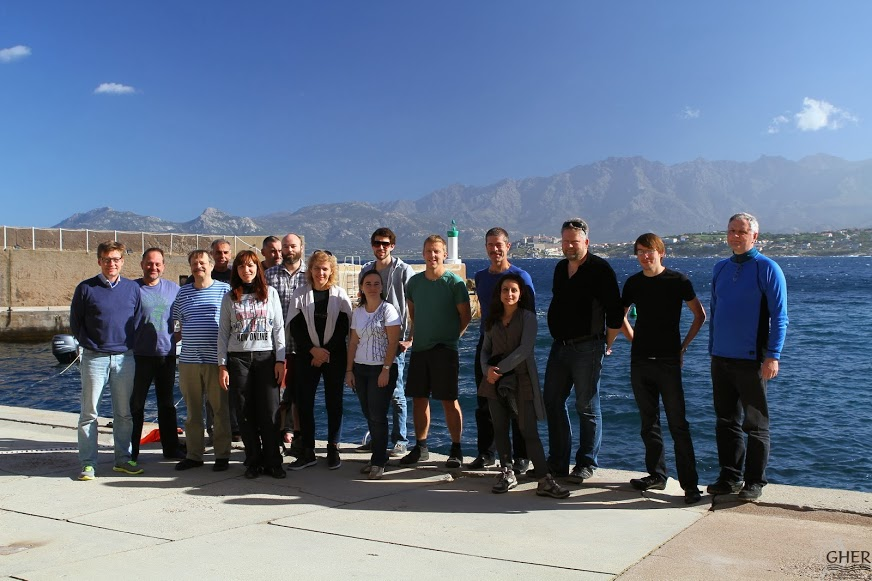
\includegraphics[width=.7\paperwidth]{workshop2013}
\end{figure}

\end{frame}
%------------------------------------------------------------------------------------------------------------
\begin{frame}
 \frametitle{What is new since Stareso 2013 ?}
 \framesubtitle{Website informations}
 \begin{itemize}
  \item The website is often upgraded (Diva last version, updated documentation,...)
  \item History of new features and bug fixes is now available at : \url{http://modb.oce.ulg.ac.be/mediawiki/index.php/New_Diva_Features}
  \item Diva (4.6.5) on VirtualBox is now available here : \url{http://modb.oce.ulg.ac.be/mediawiki/index.php/New_Diva_Features}
  \end{itemize}
\end{frame}
%------------------------------------------------------------------------------------------------------------
\begin{frame}
 \frametitle{What is new since Stareso 2013 ?}
 \framesubtitle{Diva-4.6.4}
 \begin{itemize}
  \item Released in February 2014
  \item New features
  \begin{itemize}
  \item Introduction of logit transformation
  \item Use of a mask file to introduce a relative correlation length field in Diva2D 
  \end{itemize}
  \item Bug fixes
  \begin{itemize}
  \item Minor bug corrections following the Diva workshop 
  \end{itemize}
  \end{itemize}
\end{frame}
%-----------------------------------------------------------------------------------------------------------
\begin{frame}
 \frametitle{What is new since Stareso 2013 ?}
 \framesubtitle{Details about log and logit transformations}
 \vspace{-3mm}
 \begin{figure}
 \centering
 \caption{Salinity analysis from Example4D data}
 \vspace{-3mm}
 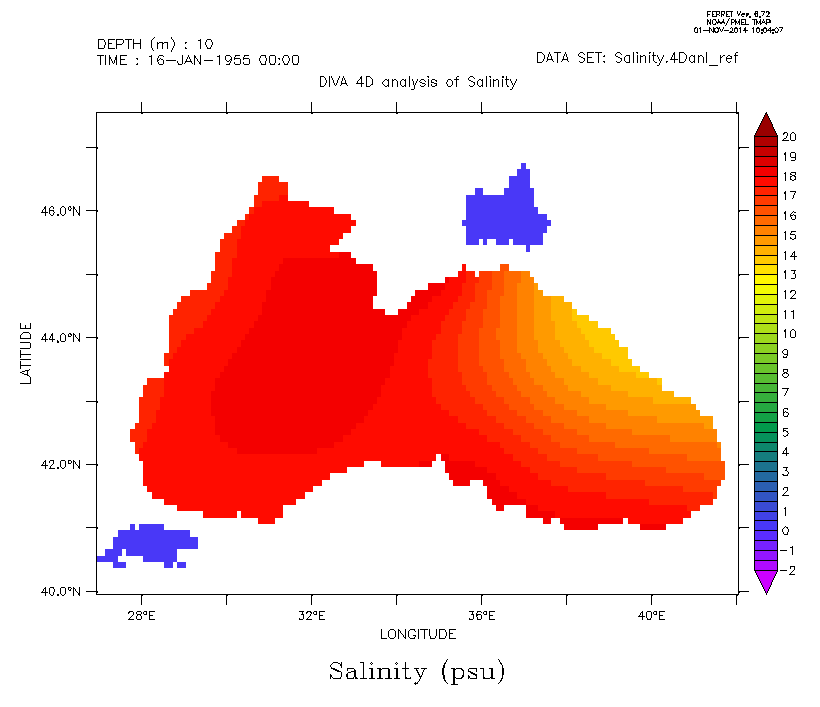
\includegraphics[width=.7\paperwidth]{salinity_ref.png}
 \end{figure}
\end{frame}
%-----------------------------------------------------------------------------------------------------------
\begin{frame}
 \frametitle{What is new since Stareso 2013 ?}
 \framesubtitle{Details about log and logit transformations}
  \vspace{-3mm}
 \begin{figure}
 \centering
 \caption{Salinity analysis modified with zeros : test}
  \vspace{-3mm}
 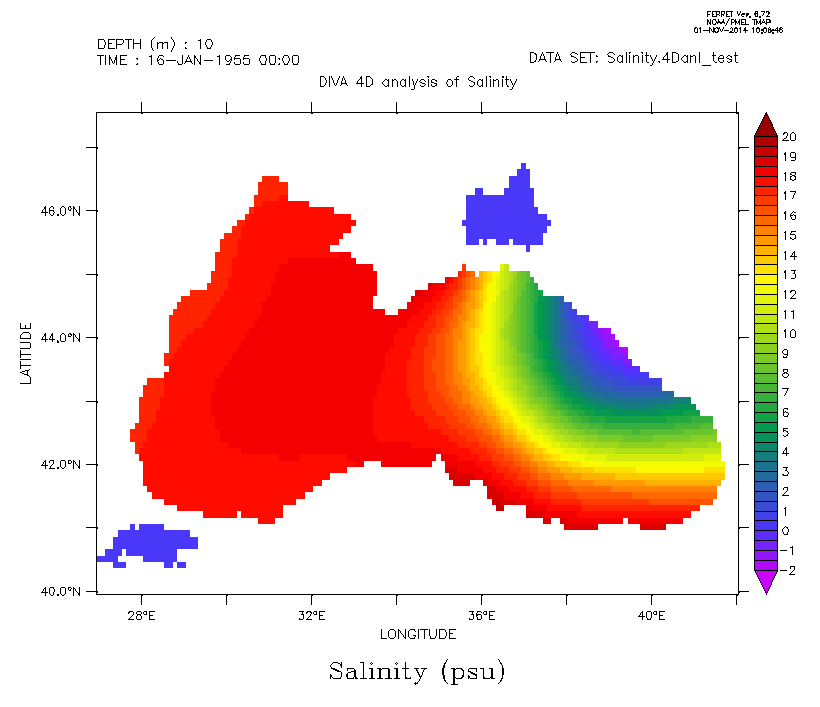
\includegraphics[width=.7\paperwidth]{salinity_test.png}
 \end{figure}
\end{frame}
%-----------------------------------------------------------------------------------------------------------
\begin{frame}
 \frametitle{What is new since Stareso 2013 ?}
 \framesubtitle{Details about log and logit transformations}
 \vspace{-3mm}
 \begin{figure}
 \centering
  \caption{Test with log transformation}
   \vspace{-3mm}
 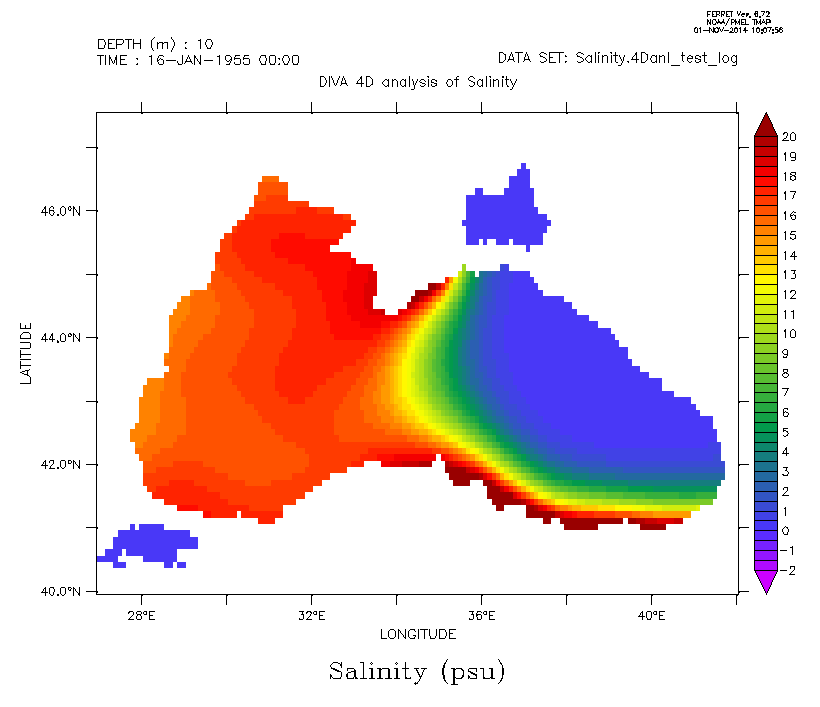
\includegraphics[width=.7\paperwidth]{salinity_test_log.png}
 \end{figure}
\end{frame}
%-----------------------------------------------------------------------------------------------------------
\begin{frame}
 \frametitle{What is new since Stareso 2013 ?}
 \framesubtitle{Details about log and logit transformations}
   \vspace{-3mm}
 \begin{figure}
 \centering
  \caption{Test with logit transformation}
   \vspace{-3mm}
 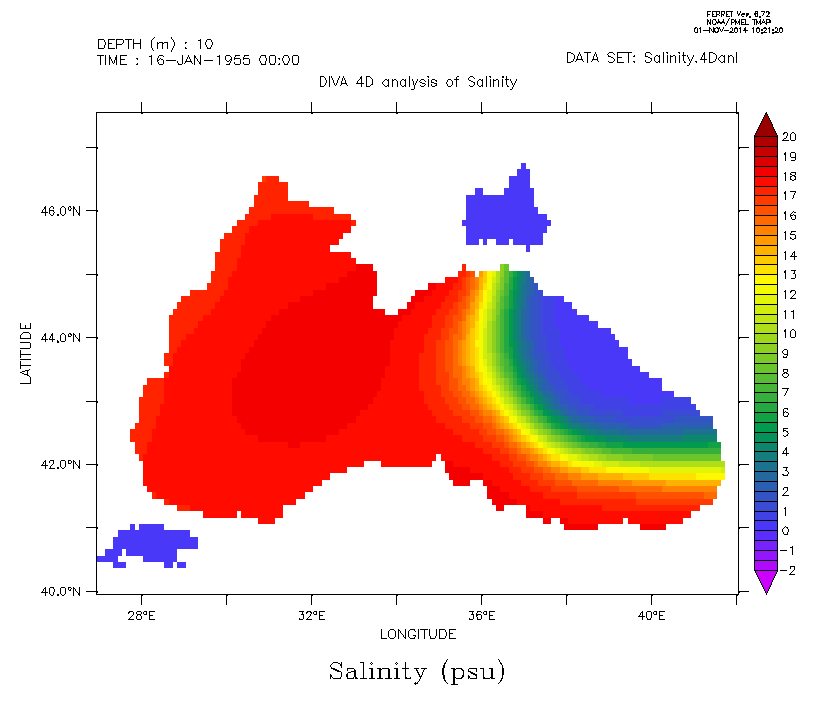
\includegraphics[width=.7\paperwidth]{salinity_test_logit_novalue.png}
 \end{figure}
\end{frame}
%-----------------------------------------------------------------------------------------------------------
\begin{frame}
 \frametitle{What is new since Stareso 2013 ?}
 \framesubtitle{Details about log and logit transformations}
   \vspace{-3mm}
 \begin{figure}
 \centering
  \caption{Test with logit transformation + logitrange (0-35)}
   \vspace{-3mm}
 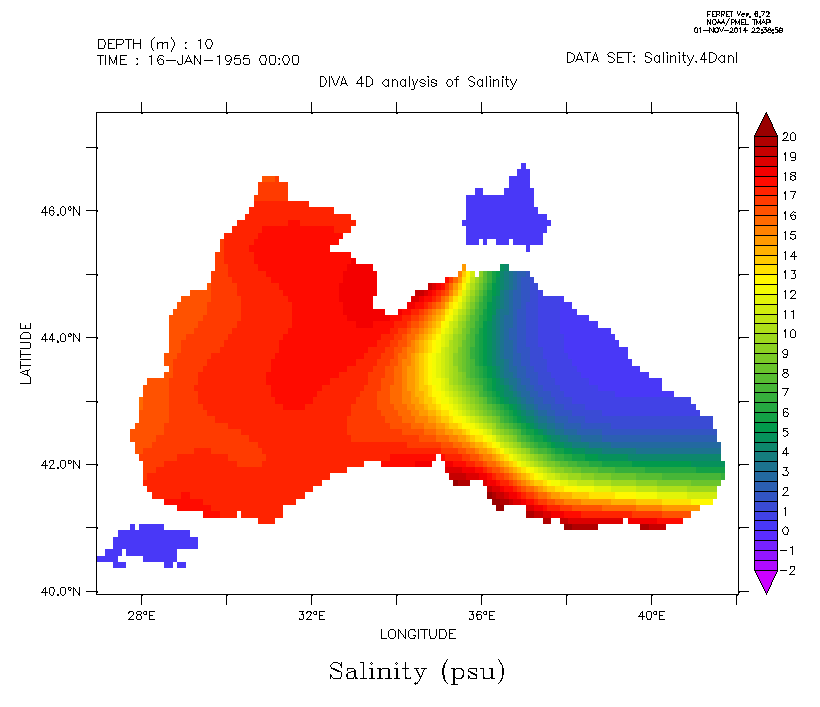
\includegraphics[width=.7\paperwidth]{salinity_test_logit_035.png}
 \end{figure}
\end{frame}
%-----------------------------------------------------------------------------------------------------------
\begin{frame}
 \frametitle{What is new since Stareso 2013 ?}
 \framesubtitle{Details about log and logit transformations}
   \vspace{-3mm}
 \begin{figure}
 \centering
  \caption{Test with logit transformation + logitrange (15-35)}
   \vspace{-3mm}
 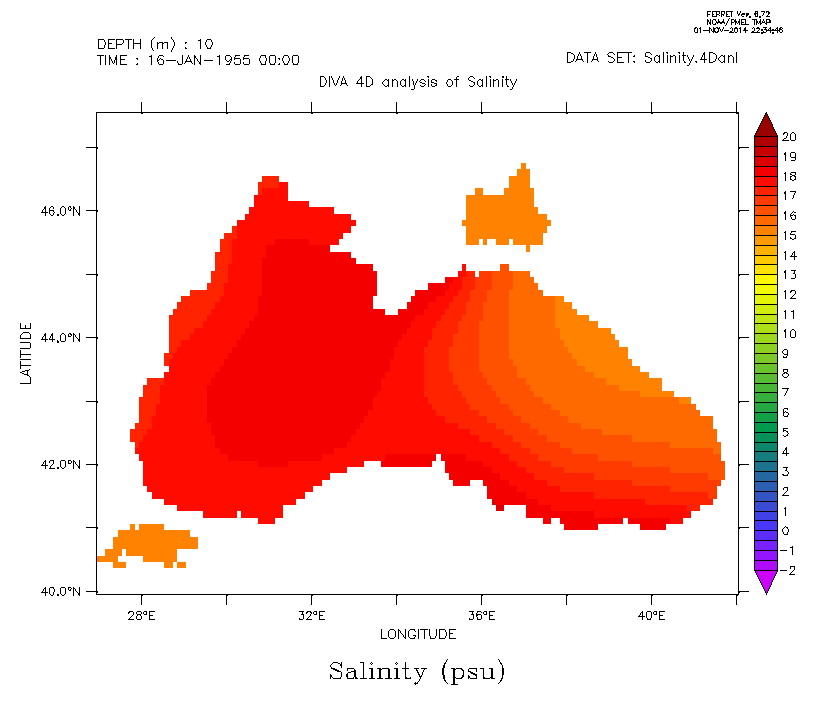
\includegraphics[width=.7\paperwidth]{salinity_test_logit_1535.png}
 \end{figure}
\end{frame}
%------------------------------------------------------------------------------------------------------------
\begin{frame}
 \frametitle{What is new since Stareso 2013 ?}
 \framesubtitle{Diva-4.6.5}
 \begin{itemize}
  \item Released in April 2014
  \item Bug fixes
  \begin{itemize}
  \item "end of line" problems under Windows (file "datasource")
  \item Portability of scripts using the "sort" command
  \item Vertical filtering of correlation length : case of 1 and 2 layer(s) 
  \item Wrong min and max values in the netcdf output file (error and analyzed field) when using some values of ispec
  \item Error field not written in the netcdf output file under some values of ispec  
  \item Other small fixes   
  \end{itemize}
  \end{itemize}
\end{frame}
%------------------------------------------------------------------------------------------------------------
\begin{frame}
 \frametitle{What is new since Stareso 2013 ?}
 \framesubtitle{Diva-4.6.6}
 \begin{itemize}
  \item Released in September 2014
  \item New features
  \begin{itemize}
   \item Check for severe errors in DIVA 3D/4D (script "godiva") + simple errors and warnings
   \item Possibility of binning the data before the parameters estimation (script "divabin" + program "binning\_lines.f90")
   \item Variable correlation length, depending on depth (script "divarlvardepth" + program "rlvardepth.f90")
  \end{itemize}
  \item Bug fixes
  \begin{itemize}
  \item Correction of the example in 4D (datasource)
  \item Correction of the script divaguessformODV4
  \item Exact match needed between variable name in "varlist" and its real name in the data file.   
  \end{itemize}
  \end{itemize}
\end{frame}
%------------------------------------------------------------------------------------------------------------
\begin{frame}
 \frametitle{What is new since Stareso 2013 ?}
 \framesubtitle{Diva on VirtualBox}
  \begin{itemize}
   \item Released in September 2014
   \item Advantages
   \begin{itemize}
   \item Diva ``ready to run'' !
   \item Works on every host system
   \item Very easy to install
   \item PATH is already ok, as well as netcdf libraries,...
   \end{itemize}
   \item Disadvantages
   \begin{itemize}
   \item Can be very slow with certain host systems / virtualbox parameters
   \item Constraints linked to use of VirtualBox (shared folders, disk space,...)
   \end{itemize}
   \end{itemize}
  Installation in 5 easy steps ? $\Rightarrow$ \url{modb.oce.ulg.ac.be/mediawiki/upload/DIVA/notes/virtualbox.pdf}
\end{frame}
%------------------------------------------------------------------------------------------------------------
\begin{frame}
  \frametitle{What is new since Stareso 2013 ?}
  \framesubtitle{Diva-4.6.7}
  \begin{itemize}
   \item Released in October 2014
   \item New features
   \begin{itemize}
   \item Transformation of user relative length or advection fields files (ascii format) into the gher binary format, via a run of Diva (new script "asctobin") 
   \end{itemize}
   \item Bug fixes
   \begin{itemize}
   \item Correction of time axis and climatology bounds in Netcdf output files %(diva3Dwrt.F,diva4Dwrt.F,dv4DYRwrt.F,dv3DncYRw.F)
   \item Correction of some attributes in 4D netcdf (databins, snr, cl, varbak) %(dv3DncYRw.F, diva3Dsub)
   \item Update of driver files (also in Example4D)   
   \end{itemize}
   \end{itemize}
\end{frame}
%------------------------------------------------------------------------------------------------------------
\begin{frame}
  \frametitle{The Diva team supports its users, everywhere in the world...}
  \pause
  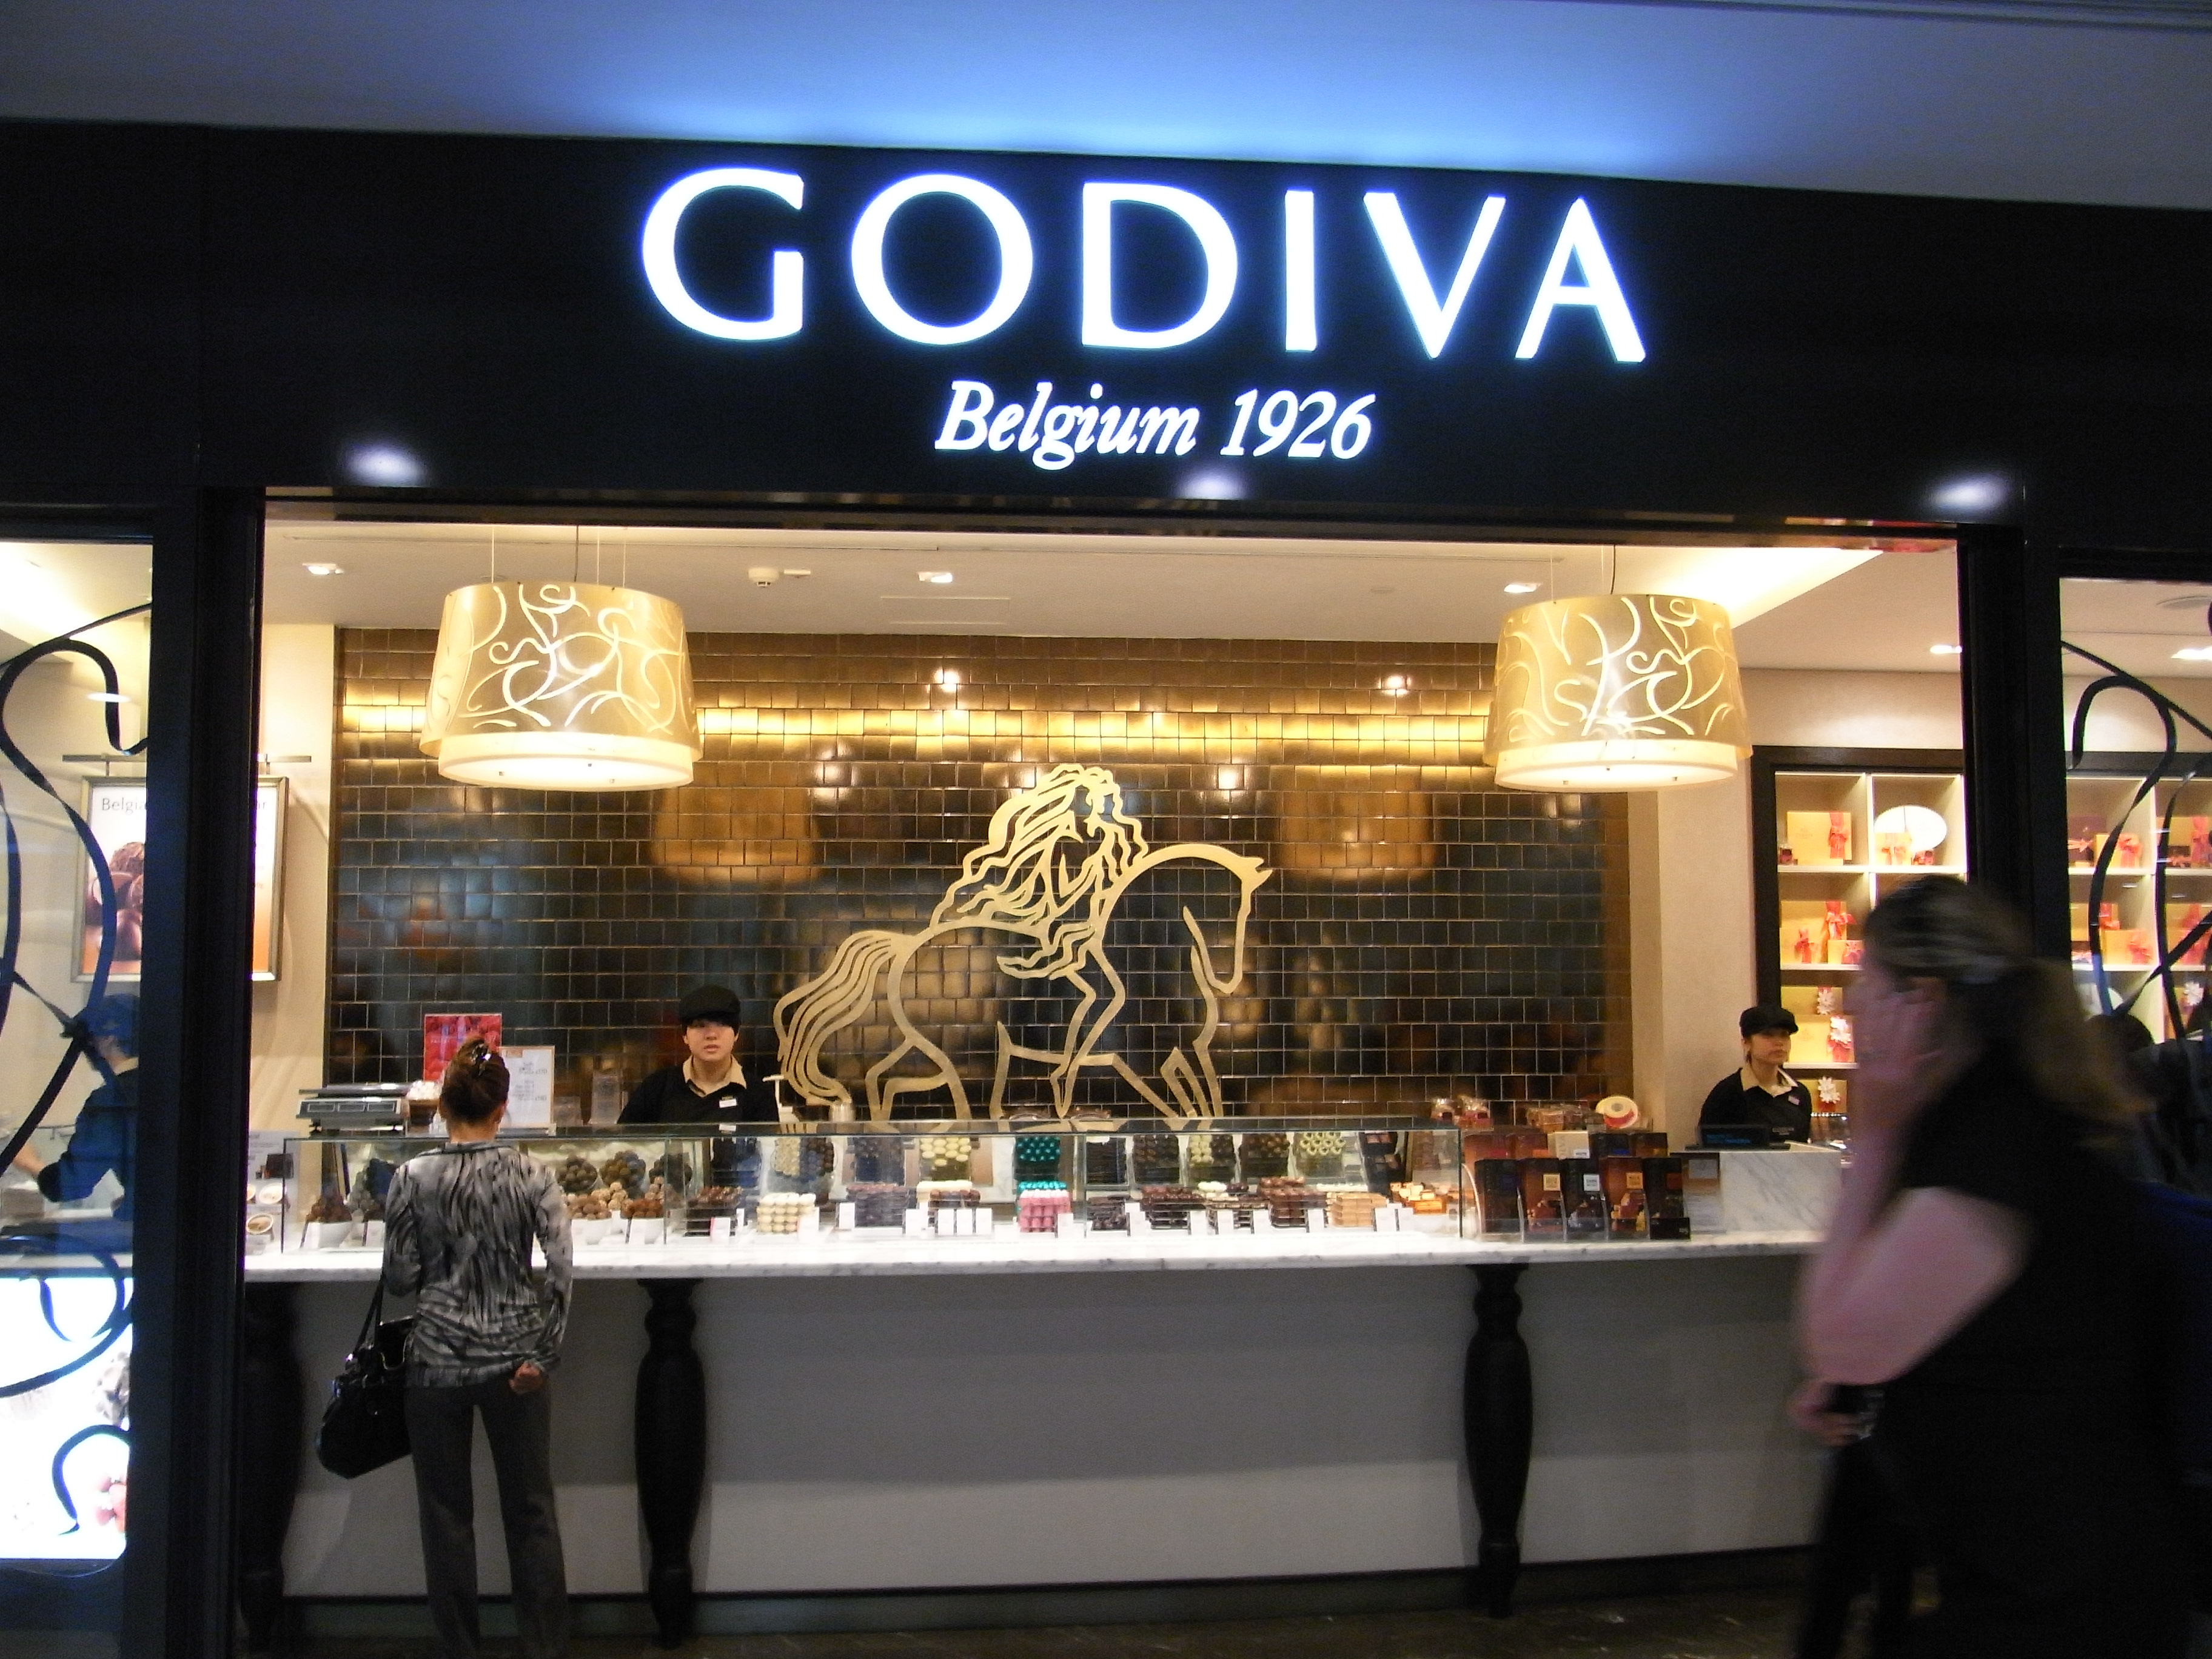
\includegraphics[scale=0.07]{./figures/HK_Central_IFC_Mall_lunch_time_shop_GODIVA_Belgium_1926_sign_April-2012.JPG}
  ~\\
   ... with chocolates.
\end{frame}
% -------------------------------------------------------------------------------------------------------------------------------------

\begin{frame}[t]
\frametitle{Releases: 4.7.1 -- expected December 2014}



\onslide*<1>{
Beta testers \ldots
\begin{figure}
\centering

\includegraphics[width=.5\paperwidth]{beta-testers}
\end{figure}
}
\onslide*<2->{
\important{Developed features}
}
\begin{itemize}
\item<2-> Correlated observational errors
\item<3-> Better file structures\\
\onslide*<3>{
\footnotesize (input and driver better separated from command) in 4D loops
}
\item<4-> Automatic selection of solver (parallel, serial, iterative)\\
\onslide*<4>{
\footnotesize depending on the problem type and size
 }
\item<5-> Retrieval of topographies from \diva-on-web 
\item<6-> Improved version of the almost exact error calculation\\
 with boundary effects
\item<7-> Incorporation of metadata \\
\onslide*<7>{
\footnotesize (EDMO-CDI identifier, space-time location)\\
 into 4D NetCDF files of climatologies
 }
\item<8-> Update of divadoxml with new template and graphic user interface (see other presentation)
\end{itemize}

\end{frame}

% -------------------------------------------------------------------------------------------------------------------------------------
\end{document}
